\chapter{Einleitung}
Dieses Dokument dient der genaueren Beschreibung und Dokumentation des Entwurfs zum Visualisierungstool \gls{programname}, dessen Hauptaufgabe die Darstellung des Netzwerkverkehrs eines \gls{profinet}-Systems ist. Des Weiteren wird der im \gls{ids} \gls{snort} eingebaute \gls{praeprozessor} \gls{sppname} und die genaue Funktionsweise der \gls{ipc} zu \gls{programname} erläutert.\newline
 \newline
Der Entwurf von \gls{programname} baut auf das klassische \gls{mvc} Design auf, welches bereits im Pflichtenheft präsentiert wurde. Abbildung~\ref{fig:arch_diagram} zeigt den erweiterten Aufbau des \gls{mvp} Musters und den detaillierteren Aufbau des Profinet Präprozessors. Im Folgenden wird auf die einzelnen Komponenten dieses Diagramms genauer eingegangen.\newline

\textbf{MODEL} (Kapitel~\ref{subsec:model}):\newline
Wie im traditionellen \gls{mvc} Muster dient das Model ausschließlich zur Speicherung von Daten in geeigneten Datenstrukturen. Im Fall von \gls{programname} umfasst dies den Graphen (Kapitel~\ref{subsubsec:graph}), die Programmeinstellungen (Kapitel~\ref{subsubsec:configdata}), Filter (Kapitel~\ref{subsubsec:filter}) und das Graphdatenlog (Kapitel~\ref{subsubsec:graphlog}). Der Benachrichtigungspfeil vom Model ausgehend bedeutet, dass bei Veränderung des Models eine Nachricht an alle Listener geschickt wird die unter Verwendung des Frameworks mit dem Model in Kontakt stehen.\newline
 \newline
\textbf{VIEW} (Kapitel~\ref{subsec:view}):\newline
Auch der View unterscheidet sich kaum von der ursprünglichen Funktionalität. Er dient weiterhin dazu, dem Benutzer eine Plattform zur Interaktion mit dem Programm zu bieten. Ein wesentlicher Unterschied zum ursprünglichen Aufbau ist hierbei jedoch, dass der View nur spezifische Interaktionen (siehe Kapitel~\ref{subsec:interaction}: interaction) kennt und ausführen kann. Wobei der View keine Kenntnis über die hinter der Aktion stehende Logik hat. Nach dem Ausführen einer Aktion wird das damit verknüpfte Command über das Notification Framework zu den \gls{listener}n geschickt. Somit nutzt der View das Notification Framework einerseits, um Benutzereingaben als Events zum Service weiterzuleiten und andererseits um Benachrichtigungen über die Zustandsveränderung des Models zu erlangen.\newline
 \newline
\textbf{INTERACTIONS} (Kapitel~\ref{subsec:interaction}):\newline
Wie bereits im vorherigen Absatz beschrieben, dienen Interaktionen dem View als Verknüpfung zwischen den tatsächlich ausgeführten Commmands und den Nutzerinteraktionen.\newline
 \newline
\textbf{COMMANDS} (Kapitel~\ref{subsec:command}):\newline
Commands enthalten neben dem service Package den Großteil der Programmlogik. Nur Commands haben die Möglichkeit Veränderungen am Model vorzunehmen, was durch den roten \textit{manipulieren} Pfeil dargestellt ist. Wenn Commands nach Eingaben des Benutzers ausgeführt werden sollen, werden diese nicht direkt referenziert sondern nur die damit verbundenen Interaktionen.\newline
 \newline
\textbf{PRESENTER} (Kapitel~\ref{subsec:presenter}):\newline
Der Presenter leistet die gesamte Aufbauarbeit. Commands werden mit bestimmten Interaktionen verknüpft, grafische Oberflächen werden instanziiert und vorbereitet und das Modell wird erstellt. 
Zusätzlich kümmert sich der Presenter um den Start sämtlicher Service Routinen und die Initialisierung des Notification Frameworks. Letzteres ist im Diagramm nicht explizit dargestellt.\newline
 \newline
\textbf{SERVICE} (Kapitel~\ref{subsec:service}):\newline
Die Bestandteile des service Packages sind eigenständige Programmroutinen. Entkoppelt von dem Rest des Programms erledigen sie Aufgaben und können mittels des Notification Frameworks mit neuen Aufgaben und Informationen versorgt werden.\newline
 \newline
\textbf{NOTIFICATION FRAMEWORK} (Kapitel~\ref{subsec:util}):\newline
Das Notification Framework dient zur Kommunkation zwischen den einzelnen Programmteilen und ermöglicht dabei den Aufbau einer entkoppelten Logik.\newline
 \newline
\textbf{SNORT} (Kapitel~\ref{sec:spp_arch} und~\ref{sec:spp_sq}):\newline
Innerhalb Snorts erfolgt der Ablauf wie folgt: Snort initialisiert den Präprozessor, wodurch dieser den Server aufbaut und als neuen Thread für einen Client abrufbar macht. Während des Programmablaufs übergibt Snort die intern dekodierten Pakete an den Präprozessor. Dieser nutzt die Dissector Struktur um das Paket zu dekodieren. Im Anschluss wird aus dem dekodierten Paket ein \gls{truffle} mit speziellen Informationen erstellt, welches dem Client über die Serververbindung bereitgestellt wird.\newline

\begin{sidewaysfigure}
  \centering
  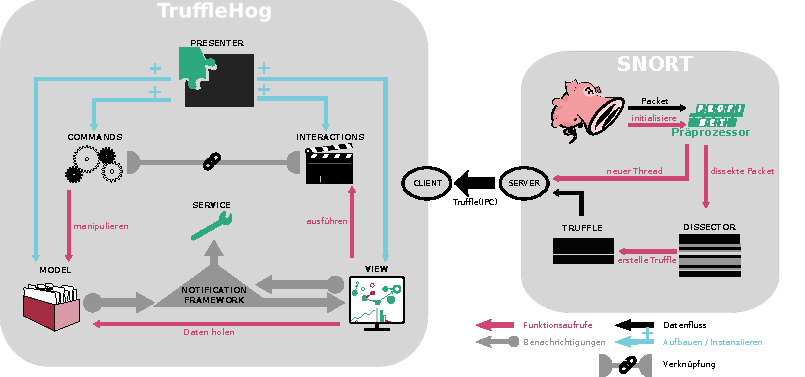
\includegraphics[width=\textwidth]{../diagramimages/arch_diagram_mvp.pdf}
  \caption[Erweiterte Architekturübersicht]{Erweiterte Architekturübersicht}
  \medskip
  Erweiterte Strukturierung des Programms nach dem \gls{mvp} Muster
  \label{fig:arch_diagram}
\end{sidewaysfigure}
\FloatBarrier
